\documentclass[a4paper,11pt]{article}
\author{Quelli della B1}
\usepackage[utf8]{inputenc}
\usepackage[italian]{babel}
\usepackage{graphicx}
\usepackage[colorlinks=true,linkcolor=blue]{hyperref}
\usepackage{hyperref}
\usepackage{nameref} 
\graphicspath{{./images/}}

\def\code#1{\texttt{#1}}
\def\sec#1{\section{#1}\label{#1}} 
\def\sub#1{\subsection{#1}\label{#1}} 
\def\subsub#1{\subsubsection{#1}\label{#1}} 
\def\vedi#1{\nameref{#1}} 

\title{Networking}

\begin{document}

\maketitle
\newpage
\tableofcontents
\newpage

\sec{Introduzione}
%quattro parole sulla storia del networking
\sub{Organizzazioni}
\subsub{IEEE}
\subsub{CCITT - ITU}
\subsub{ISO}
\subsub{IETF}
Internet Engineering Task Force:
%Gioara 
\sub{Il modello di riferimento ISO/OSI}
Il modello Open Systems Interconnection (abbreviato in modello ISO/OSI) è stato progettato dall’International Organization for Standardization (ISO) come modello di riferimento per consentire una comunicazione aperta tra diversi sistemi tecnici. Questo punto diventa più chiaro, se si pensa alle origini di Internet: alla fine degli anni ’70 i leader del settore nelle tecnologie di rete si ritrovarono di fronte al problema che le architetture di rete proprietarie si potevano collegare solo tramite dispositivi propri, infatti nessun produttore aveva pensato di costruire componenti hardware o software compatibili con le specificazioni di altri fornitori. Ma un progetto come quello di Internet presuppone alcuni standard per poter rendere possibile una comunicazione comune.
Il modello lSO/OSI è nato dal tentativo di creare uno standard di questo tipo e offre una base per gli standard di comunicazione, indipendentemente dai fornitori. In base a questo modello, il complesso processo della comunicazione di rete si divide in sette strati, i livelli (in inglese layer). Si parla perciò anche di una comunicazione per livelli. All’interno della comunicazione tra due sistemi devono essere svolti degli specifici compiti su ogni singolo livello, tra questi rientrano ad esempio il controllo della comunicazione, l’indirizzamento del sistema target o la conversione dei pacchetti in segnali fisici. Ma questo funziona solo se tutti i sistemi coinvolti nella comunicazione si attengono a regole precise, stabilite nei protocolli, che si applicano ai singoli livelli o si possono utilizzare su ciascuno di questi (multilivello).
\\Il modello di riferimento ISO/OSI non è però uno standard di rete concreto, ma descrive in forma astratta quali procedimenti devono essere regolati per far funzionare la comunicazione in una rete.  
\subsub{I livelli}
La comunicazione tra due computer può apparire banale agli utenti, ma in realtà durante la trasmissione di dati in una rete devono essere compiuti numerosi compiti e soddisfatte diverse richieste nell’ambito dell’attendibilità, della sicurezza e dell’integrità. Per questo si è deciso di dividere la comunicazione di rete in livelli. Ad ogni livello, strutturato gerarchicamente, sono assegnate delle funzioni specifiche (quindi uno standard copre generalmente solo una parte del modello): ogni livello accede tramite un’interfaccia a quello inferiore e mette a disposizione il servizio del livello superiore.
\\Questo principio ha due vantaggi decisivi:
\begin{itemize}
	\item I compiti e le richieste che devono essere compiuti e soddisfatti all’interno di un livello sono definiti chiaramente. Per ogni livello possono essere sviluppati degli standard indipendenti gli uni dagli altri.
	\item La chiara divisione tra i singoli livelli fa sì che le modifiche ad uno standard non abbiano alcun effetto sui processi che si svolgono su un altro livello. Introdurre nuovi standard risulta così più semplice.
\end{itemize}
I sette livelli del modello ISO/OSI si dividono in due gruppi in base ai compiti che svolgono: orientati all’applicazione e orientati al trasporto. I processi che si svolgono sui singoli livelli si possono spiegare prendendo ad esempio la trasmissione e-mail da un dispositivo ad un mail server.

\sub{Internet protocol suite (TCP/IP)}


\sub{Standardizzazione}
%definizione di 'standard'
\subsub{IEEE 802}
\subsub{RFC}
Request For Comments: documento pubblicato dalla \vedi{IETF} riportante informazioni o specifiche riguardanti innovazioni nell'ambito di \vedi{Internet}. Fonte ufficale: \url{rfc-editor.org}
\newpage

\sec{Livello Fisico}
Nonostante l'amministratore di rete non abbia la possibilità di influirvi direttamente, è importante descrivere lo strato fisico poiché esso influenza significativamente le prestazioni della rete.

\subsection{Terminologia}
\subsub{Informazione} 
L'informazione è una grandezza misurabile in bit. In particolare, \[Q=log_{2}m\] dove $Q$ è il numero di bit necessari per rappresentare l'informazione relativa ad $m$ possibili stati.

\subsub{Codice}
Al fine di rappresentare l'informazione in maniera tale da renderne più semplice la gestione, un codice associa sequenze di bit a caratteri. I codici che godono della più ampia diffusione sono:
\begin{itemize}
\item ASCII (American Standard Code for Information Interchange, 7 bit estesi a 1 byte)
\item BCD (Binary-Coded Decimal)
\item AIKEN 
\item Gray
\item EBCDIC (Extended Binary Coded Decimal Code, 8 bit), in uso presso le banche
\end{itemize}

\subsub{Segnale}
Si dice \textit{segnale} una grandezza fisica variabile nel tempo corrispondente un'informazione. Un segnale \textbf{analogico} varia in modo continuo nel tempo ed ha infiniti livelli di intensità; un segnale \textbf{digitale} varia invece in modo discreto e ha solo due livelli di intensità. Ogni tipo di dato può essere rappresentato in entrambe le maniere e può essere convertito da analogico a digitale e viceversa.
\\\\Fra i segnali analogici assumono particolare rilevanza i \textbf{segnali sinusoidali}, ossia segnali che variano nel tempo secondo una legge del tipo \[u=Usen(\omega t+\Phi )\] dove 
\begin{itemize}
\item $u$ è l'ampiezza istantanea
\item $U$ è l'ampiezza massima
\item $\omega $ è la velocità angolare 
va spiegato meglio
\item $\Phi $ è lo sfasamento rispetto all'origine
\item l'intervallo di tempo impiegato dall'onda per tornare allo stesso livello d'intensità è detto \textit{periodo}.
\item $1/t=f$ è detta \textit{frequenza} (misurabile in Hz)\\\\
\end{itemize}
La curva in figura rappresenta istante per istante il valore del seno dell'angolo descritto da un segmento che ruota con un estremo vincolato all'origine degli assi cartesiani, in senso antiorario, con velocità angolare $\omega $. Di conseguenza, la frequenza $f$ è il numero di volte che il segmento effettua un giro completo.
\begin{figure}
\centering
\fbox{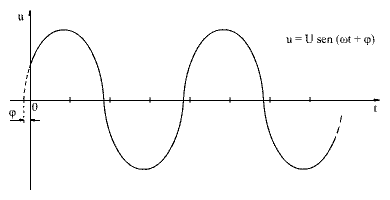
\includegraphics[scale=0.5]{segnali_sin.png}}
\caption{Rappresentazione grafica di un segnale sinusoidale}\label{fig. 1}
\end{figure}

\subsubsection{Lunghezza d'onda}
In un segnale sinusoidale, la distanza tra due massimi relativi è detta \textit{lunghezza d'onda} $\lambda =c/f$ (dove $c$ è la velocità di propagazione del segnale).

\subsub{Spettro}
Lo spettro è l'insieme delle frequenze che compongono un segnale. Questa affermazione, non necessariamente di immediata comprensione, diventa subito chiara se si tiene presente il \textbf{teorema di Fourier}, il quale afferma che un segnale può essere rappresentato come somma di sinusoidi (potenzialmente infinite) con caratteristiche differenti.

\subsub{Ampiezza di banda}
L'ampiezza di banda è costituita dall'insieme di frequenze dello spettro \textit{effettivamente utilizzate} e corrisponde alla massima velocità teorica della rete. Si parla di \textit{banda larga} nel caso in cui l'ampiezza di banda sia sensibilmente superiore a quella utilizzata correntemente per le comunicazioni telefoniche.

\subsection{Qualità delle trasmissioni}
Come già accennato in precedenza, é lo strato fisico che determina in larga parte la qualità delle comunicazioni, valutabile in base a prestazioni e affidabilità. 
\\Vi sono numerosi strumenti software per valutare la qualità di una rete, quali:
\begin{itemize}
\item il comando Unix \code{ping}, che indica se un host remoto possa essere raggiunto e riporta statistiche sui pacchetti persi
\item il comando Unix \code{traceroute} o \code{tracepath}, che indica i dispositivi attraversati per raggiungere una data destinazione
\item applicazioni web quali ad esempio \url{speedtest.net} e \href{<https://www.misurainternet.it/>}{Ne.Me.Sys}, quest'ultimo sviluppato da AGCOM, i cui risultati possono essere utilizzati come elemento probatorio nel caso in cui l’utente voglia esercitare il diritto di reclamo e recesso rispetto a promesse contrattuali di velocità di accesso ad Internet non mantenute dall‘operatore.
\end{itemize}

\subsub{Criteri di valutazione in base alle prestazioni}
\begin{itemize}
\item \textbf{ritardo}: tempo necessario per il transito dei dati
\item \textbf{tempo di risposta}: tempo che intercorre tra il momento in cui viene effettuata una richiesta e il momento in cui si ottiene una risposta
\item \textbf{throughput}: quantità di dati spedita nell'unità di tempo; rappresenta l'effettiva velocità della rete
\item \textbf{latenza}: tempo necessario perché un messaggio giunga a destinazione; per il suo calcolo si tiene conto di:
\begin{itemize}
\item \textbf{tempo di propagazione}: tempo di transito sulla rete per arrivare dal mittente al destinatario
\item \textbf{tempo di trasmissione}: tempo necessario per immettere i bit sulla rete, ossia $\frac{dim_{m}}{v}$, dove $dim_{m}$ è la dimensione del messaggio e $v$ la velocità trasmissiva
\item \textbf{tempo di inoltro}: tempo necessario ai nodi per consegnare il messaggio in transito, non legato al traffico ma solo ad hardware e software
\item \textbf{tempo di attesa} nelle code di rete, dipendente dal traffico
\end{itemize}
\subsubsection{Criteri di valutazione in base all'affidabilità}
\item \textbf{jitter}: variabilità del ritardo con cui i pacchetti vengono consegnari in ricezione
\item \textbf{packet loss}: pacchetti persi.

\sub{Filtri}
\end{itemize}
Un filtro è un sistema che tratta le varie componenti del segnale in modo diverso a seconda della loro frequenza.
\\E' opportuna innanzitutto una distinzione tra filtri \textit{passivi} ed \textit{attivi}: i primi sono costituiti solamente da resistenze e condensatori, mentre i secondi includono altre componenti, come i transistor e gli amplificatori. Inoltre, a seconda del comportamento, si distinguono quattro tipi di filtri:
\begin{itemize}
\item \textbf{filtro passa basso}: permette il passaggio delle frequenze al di sotto di una determinata \textit{frequenza di taglio}, definita come \[\frac{v_{out}}{v_{in}}=\frac{1}{(2)^{1/2}}\]
dove $v_{in}$ è il segnale in ingresso e $v_{out}$ il segnale in uscita.
\item \textbf{filtro passa alto}: complementare al filtro passa basso, permette il passaggio delle frequenze al di sopra della frequenza di taglio, definita come sopra
\item \textbf{filtro passa banda}: composizione di un filtro passa basso e un filtro passa alto
\item \textbf{filtro elimina banda}: complemento del filtro passa banda, blocca le frequenze comprese tra due frequenze di taglio.
\end{itemize}

\sub{Modulazione}
Sovente capita che l'informazione debba essere convertita in maniera idonea ad essere inviata nel mezzo trasmissivo adottato. Tale processo è detto \textit{modulazione} ed è reversibile: il \textit{segnale portante}, caratteristico del mezzo trasmissivo, viene modificato in uno dei suoi parametri essenziali in accordo al segnale in ingresso, contenente l'informazione da trasmettersi, che è detto \textit{segnale modulante}.
\subsub{Ad onda continua}
Si parla di modulazione ad onda continua nel momento in cui viene modulata una portante sinusoidale. Ne esistono tre tipologie:
\begin{itemize}
\item \textbf{AM} (Amplitude Modulation): l'ampiezza del segnale portante viene modulata in proporzione al segnale modulante. Per quel che riguarda la trasmissione digitale, lo 0 è associato a bassa potenza e l'1 ad alta potenza.
\item \textbf{FM} (Frequency Modulation): è la frequenza del segnale portante ad essere modulata, infittendosi quando la modulante si innalza e rafefacendosi quando si abbassa. Tipica delle trasmissione radiofoniche in Italia, pur necessitando di circuiti più complessi, è preferibile alla modulazione di ampiezza per motivi di efficienza e maggior tolleranza a disturbi di vario tipo.
\item \textbf{PM} (Phase Modulation): molto simile alla modulazione di frequenza - come si può notare in figura, consiste nel variare la fase $\Phi $ (vedi \vedi{Segnale}) in proporzione all'intensità della modulante. Spesso s'impiega in sistemi in FM per ottenere l'amplificazione del segnale. 
\end{itemize}
\begin{figure}[h]
\centering
\fbox{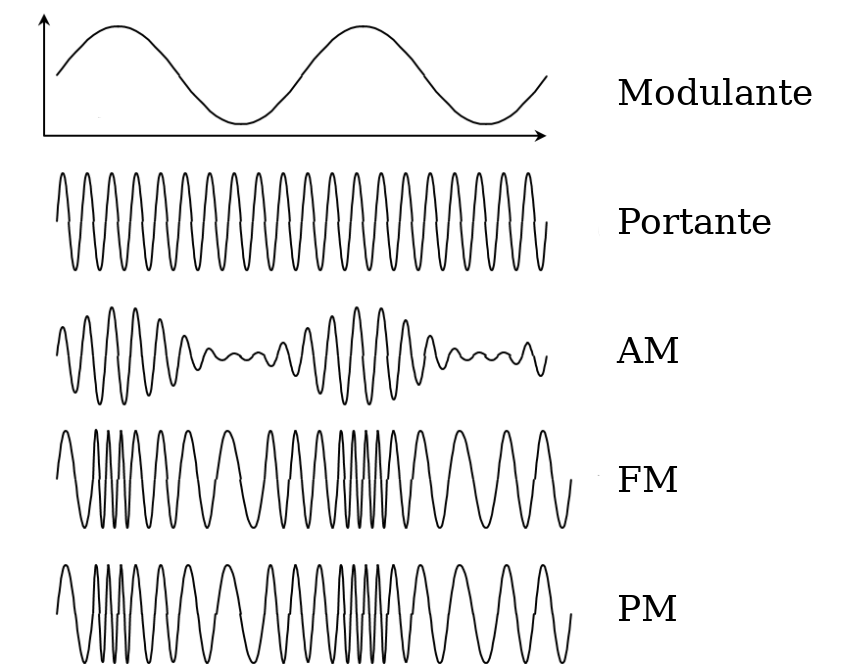
\includegraphics[scale=0.5]{am_fm_pm.png}}
\caption{Confronto tra tipologie di modulazione ad onda continua}\label{fig. 2}
\end{figure}
\subsub{Impulsiva}
La modulazione impulsiva è un tipo di modulazione in cui l'informazione è codificata in una serie di impulsi. I principali tipi di modulazione impulsiva sono:
\begin{itemize}
\item \textbf{PAM} (Pulse Amplitude Modulation), analoga alla AM
\item \textbf{PFM} (Pulse Frequency Modulation), analoga alla FM
\item \textbf{PPM} (Pulse Phase Modulation), analoga alla PM
\begin{figure}[h]
\centering
\fbox{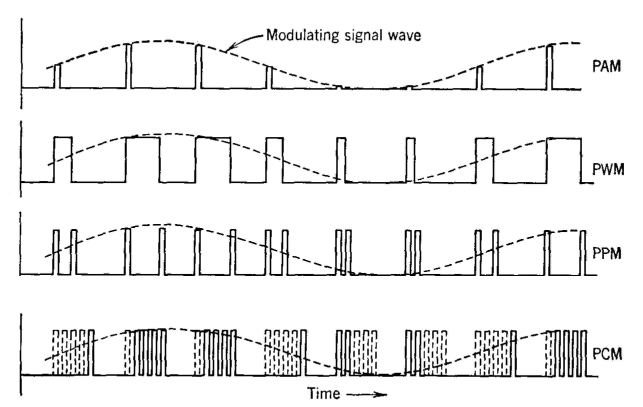
\includegraphics[scale=0.5]{pam_pwm_ppm_pcm.png}}
\caption{Confronto tra tipologie di modulazione impulsiva}
\label{fig. 3}
\end{figure}
\item \textbf{PCM} (Pulse Code Modulation), nata dall'esigenza, intorno agli anni '40, di aumentare il numero di collegamenti telefonici interurbani. Per evitare l'impianto di grossi fasci di conduttori, ingombranti, costosi e difficili da connettere, si pensò di multiplare un gran più collegamenti su un unico cavo, utilizzando una soluzione preesistente, la \textbf{FDM} (Frequency Division Multiplexing), poi  abbandonata per la più moderna \textbf{TDM} (Time Division Multiplexing), inizialmente realizzata per mezzo delle tre tecniche impulsive sopra descritte, poi attraverso appunto la PCM, ad oggi l'unica adottata su larga scala. La PCM costa di tre fasi distinte:
\begin{itemize}
\item \textbf{campionamento}: conversione del segnale continuo in un segnale discreto nel tempo, valutandone l'ampiezza a intervalli di tempo regolari. Ciò è possibile, come affermato dal \href{<https://it.wikipedia.org/wiki/Teorema_del_campionamento_di_Nyquist-Shannon>}{Teorema di Shannon}, poiché è possibile rappresentare un segnale con frequenza limitata tra $f_{1}$ ed $f_{2}$, con $f_{1}<f_{2}$ mediante una successione di campioni con frequenza minima $2f_{2}$. La minima frequenza di campionamento (\textbf{cadenza di Nyquist}) è pari al doppio della banda; nella PSTN (Public Switched Telephone Network) si assume come frequenza di campionamento $f_{c}=8 Khz$.
\item \textbf{quantizzazione}: conversione di un segnale a valori continui in uno a valori discreti. Per ottenere un range di valori discreti, si stabiliscono un valore minimo e un valore massimo e si suddivide l'intervallo così ottenuto. Nella quantizzazione uniforme, l'ampiezza è uguale per tutti i sottolivelli; di norma, tuttavia, essa segue una scala logaritmica. Com'è intuibile, la quanmtizzazione è un processo irreversibile, per cui è necessario tener conto dell'errore commesso - si è verificato che, utilizzando 256 livelli di quantizzazione, l'orecchio umano non percepisce sostanziali differenze.
\item \textbf{codifica}: gli impulsi campionati e quantizzati vengono convertiti in sequenze di bit (nel PCM europeo, che utilizza appunto $256=2^{8}$ livelli, occorrono 8 bit per campione).
\end{itemize}
\begin{figure}[h]
\centering
\fbox{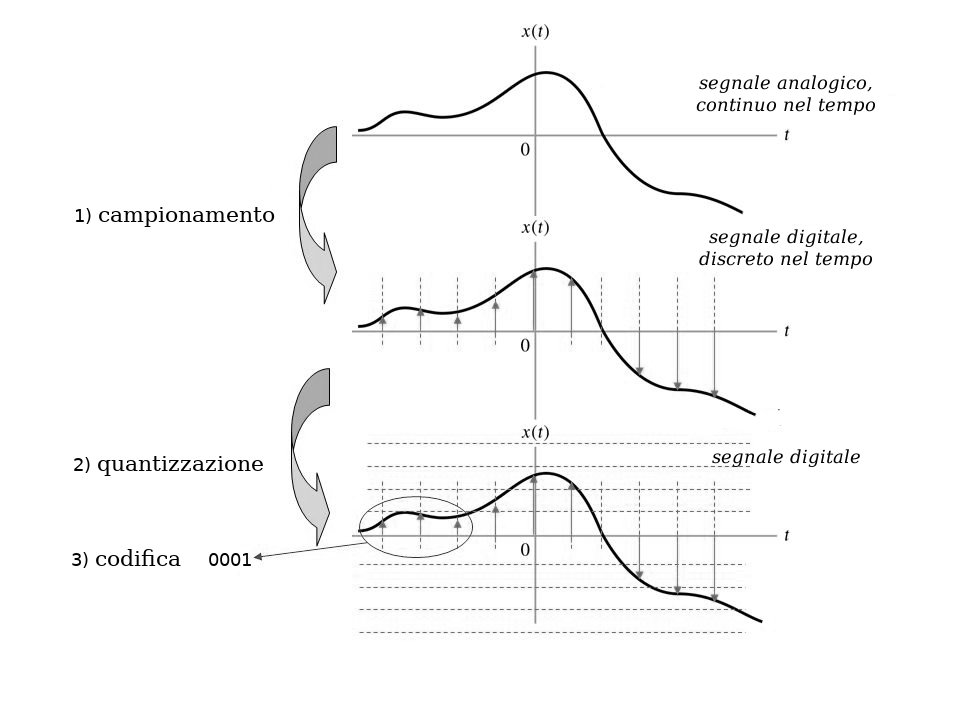
\includegraphics[scale=0.5]{pcm.jpg}}
\caption{Fasi della PCM}
\label{fig. 4}
\end{figure}
\end{itemize}

\subsub{Digitale}

\sub{Alterazioni del segnale}
\subsub{Attenuazione}
\subsub{Distorsione}
\subsub{Rumore}
\subsub{Interferenza}

\subsection{Limiti alla velocità di trasferimento}
\subsub{Classificazione dei canali trasmissivi}
\subsub{Teorema di Nyquist}
\subsub{Teorema di Shannon}
\subsubsection{Velocità di modulazione}
\newpage
\sec{Livello di Collegamento}
%Filippo---------------------------------------------------------------------------------------------------------------------
\sub{Ethernet} 
\subsub {Ethernet framing}

\sub{Tipi di trasmissione}
\subsub{Sincrona}
\subsub{Asincrona}
\subsub{Orientata al carattere}
\subsub{Orientata al bit}

\sub{Controllo degli errori}
\subsub{Ridondanza}

\sub{Flussi trasmissivi}
\subsub{Simplex}
\subsub{Half-Duplex}
\subsub{Full-Duplex}

%NB non credo vadano qui...
%\sub{Protocolli primario-secondario}
%\subsub{RTS-CTS}
%\subsub{XON-XOF}
%\subsub{ARQ}

\sub{Protocolli di collegamento con lv3} 
\subsub{ARP}
Due host internet possono comunicare solamente conoscendo il reciproco indirizzo fisico(mac address), che è specifico di ogni macchina e quindi non individuabile dall' esterno.
L' host A, per sapere l' indirizzo fisico di B, invierà una richiesta ARP (contenente IP di sia di A che di B), B la chiamata a suo nome e risponde segnando l' IP di a in una cache di consultazione e riinviando il proprio mac address a A
\subsub{RARP} 
%\subsub{NDP} 
%ARP, MAC, Ethernet da spostare nel lv. di rete?
 
\sec{Livello di Rete}
%Claudio & Giorgio ---------------------------------------------------------------------------------------------------------------------
\subsection{Terminologia}
\subsub{Rete}
Insieme di dispositivi connessi da canali di comunicazione.
\subsub{DTE}
Data Terminal Equipment: qualunque dispositivo che è la sorgente o la destinazione di una comunicazione di dati.
Un esempio è il Personal Computer (PC). 
\subsub{DCE}
Data Circuit-terminating Equipment o Data Communication Equipment: dispositivo intermedio 
tra uno o più \vedi{DTE} e il resto della rete; esegue conversioni di segnale, correzione di errori
e gestisce il clock dei dispositivi connessi. Può anche essere interno al \vedi{DTE}. Tipicamente è un Modem.
\subsub{CPE}
Customer Premises Equipment: dispositivo terminale connesso direttamente ad una \vedi{WAN}. Rientrano in questa categoria telefoni, Router e Switch di rete.

\sub{Tipologie di rete cablata}
\subsub{PAN} Personal Area Network: Rete personale come quella composta dal PC e da altri dispositivi domestici connessi tra di loro via cavo.
\subsub{LAN} Local Area Network: Rete con un raggio limitato ad una abitazione o un edificio. (La prima rete LAN è stata ARKNET nel 1977)
\subsub{WAN} Wide Area Network: Rete che copre ampie aree geografiche connettendo tra loro più sottoreti locali. 
\subsub{MAN} Metropolitan Area Network: Rete metropolitana caratterizzata da una velocità di trasmissione molto elevata (tipicamente fibra ottica).
\subsub{GAN} Global Area Network: \vedi{Internet}.

\sub{Tipologie di rete wireless}
\subsub{NFC} Near-Field Communication: Lo scambio di informazioni tramite tag elettromagnetici.\\ Portata: 20cm.
\subsub{BAN} Body Area Network: Rete che collega dispositivi indossabili, raggio di azione inferiore al metro.
\subsub{WPAN} Wireless Personal Area Network: Rete di dispositivi personali in un raggio inferiore ai 20 metri, ad esempio stampanti Bluetooth.
\subsub{WLAN} Wireless Local Area Network: LAN ottenuta tramite tegnologie wireless, ad esempio reti WiFi. 

\sub{Topologia delle reti}
\subsub{Rete a dorsale}
I dispositivi sono connessi tutti ad una via di trasmissione principale detta appunto dorsale. Un interruzzione in qualunque punto della dorsale compromette tutta la rete.
\subsub{Rete ad albero} La trasmissione avviene in modo gerarchico tra i nodi padre e figlio, fino ad arrivare alla \textit{root} dalla quale dipende tutto il funzionamento della rete.
\subsub{Rete a stella} Tutti i dispositivi sono connessi ad un HUB (router o swith di rete), più economico da sostituire in caso di rottura. Inoltre, in caso di danni ad un cavo, viene disconnesso solo un terminale. Questa topologia è tipicamente utilizzata per la realizzazione di reti \vedi{LAN}. 
\subsub{Rete ad anello} Le informazioni vengono passate da un dispositivo all'altro in modo ciclico, la trasmissione è unidirezionale anche se questo si può ovviare con un secondo anello in direzione opposta. Questa topologia era tipica delle \vedi{LAN} TokenRing, ora viene utilizzata principalmente nelle \vedi{MAN} in fibra ottica.
\subsub{Rete a maglia} In inglese \textit{mesh}, è una rete in cui ogni dispositivo può essere connesso ad ogni altro dispositivo ottenendo di fatto un grafo connesso. \'E la topologia di rete meno vulnerabile ma è poco utilizzata nelle reti cablate a causa dei costi elevati. \'E diffusa invece nelle \vedi{WLAN}, spesso nella versione \textit{ad -hoc} dove i collegamenti nascono e muoiono dinamicamente. In questa topologia il \vedi{Routing} viene effettuato da ogni nodo.

%GRID? 

\subsection{Qualità della rete} %da rivedere
\subsub{Jitter}

\sub{Internet}
Rete globale di reti che abilita i \vedi{DTE} a comunicare direttamente ed in modo trasparente ed a condividere servizi, definita formalmente nel \vedi{RFC}1122 (originariamente in \vedi{RFC}760.
\subsubsection{Internet Protocol (IP)} \label{IP}
Fornisce le funzioni necessarie per l'invio di un pacchetto di bit detto \textit{Internet datagram} da un host all'altro. Ogni nodo è identificato da un indirizzo IP.
\paragraph{Differenze tra IPv4 e IPv6}
L’IP versione 4 fornisce anche i servizi di
frammentazione e riassemblaggio di datagram,
quando la trasmissione avviene attraverso reti con
capacità di trasporto di pacchetti più piccola del
pacchetto originale (dovuto alle diverse tecnologie di
rete del passato). IP versione 6 abolisce questo
comportamento. %copiato dalle slide (da rivedere e ampliare)


\sub{Routing}
\subsub{Tabella di routing}
\code{netstat -nr}
\sub{Protocolli di routing}
\subsub{ICMP} 
\subsub{IGMP} 
\subsub{RIP} 
\subsub{OSPF} 

\newpage

\sec{Livello di trasporto}

Il protocollo ARQ è di tipo \vedi{Full-Duplex} %missing

\sub{Protocolli} 
\subsub{TCP} 
\subsub{UDP} 
\newpage

\sec{Livello delle applicazioni}
Il livello delle applicazioni racchiude tutte le applicazioni dedicate all'utente finale. 
Qui \'e dove la differenza fra protocollo e servizio si fa sempre pi\'u labile: molto spesso, la stessa parola (e.g. telnet) indica sia il protocollo, che la sua implementazione la quale, la maggior parte delle volte, \'e un comando Linux. 
\subsection{Protocolli}
%Tommaso
\subsub{Telnet e SSH} %standard odierno
\paragraph{Protocollo}
Telenet nasce come protocollo di rete per sistemi Unix in grado di gestire una comunicazione standardizzata fra due \vedi{DTE}. Principalmente, Telnet, \'e sempre stato utilizzato per fornire all'utente una sessione remota del terminale dell'host. L'host ascolta sulla porta 23 e l'utente stabilisce una connessione utilizzando il public IP, nome utente e password di un Unix user dell'host. L'unico grande problema di Telnet riguarda la sicurezza: \'e un protocollo non il criptato, ovvero la password il nome utente e tutte le altre informazioni inviate, risultano completamente chiare a qualsiasi utente estraneo alla conversazione.
SSH (SecureShell) nasce per ovviare questo problema: svolge le stesse funzioni di Telnet (standard porta 22) in maniera molto pi\'u sicura: utilizza coppie di chiavi pubbliche-private per cryptare la conversazione. L'host possiede la chiave pubblica che non \'e mai trasferita via internet e i client utilizzando la chiave privata corrispondente.
SSH \'e ormai lo standard per le connessioni da remoto. Telnet \'e ormai un servizio bloccato (nessuno permette delle connessioni di tipo telnet) ed inutilizzato.
\paragraph{Implementazione}

\subsub{FTP e SCP} %standard odierno
\subsub{BGP} 
\subsub{DHCP} %Discovering ,Offering , Codice 
\subsub{DNS} 
\subsub{HTTP/HTTPS} 
\subsub{NFS}
\subsub{SNMP} %problemi sicurezza, v3, Managment Information Base (MIB), SNMP trap per gestione imprevisti, polling orientato ai trap, Structure of Management Information (SMI) 

\end{document}
